% Created 2020-07-14 mar 15:05
% Intended LaTeX compiler: pdflatex
\documentclass[presentation,aspectratio=169]{beamer}
\usepackage[utf8]{inputenc}
\usepackage[T1]{fontenc}
\usepackage{graphicx}
\usepackage{grffile}
\usepackage{longtable}
\usepackage{wrapfig}
\usepackage{rotating}
\usepackage[normalem]{ulem}
\usepackage{amsmath}
\usepackage{textcomp}
\usepackage{amssymb}
\usepackage{capt-of}
\usepackage{hyperref}
\usepackage{khpreamble}
\usepackage{amssymb}
\DeclareMathOperator{\shift}{q}
\DeclareMathOperator{\diff}{p}
\usetheme{default}
\author{Kjartan Halvorsen}
\date{\today}
\title{Control computarizado - Asignación de polos (RST posicional)}
\hypersetup{
 pdfauthor={Kjartan Halvorsen},
 pdftitle={Control computarizado - Asignación de polos (RST posicional)},
 pdfkeywords={},
 pdfsubject={},
 pdfcreator={Emacs 26.3 (Org mode 9.3.6)}, 
 pdflang={English}}
\begin{document}

\maketitle

\section{Intro}
\label{sec:orgb33e3eb}

\begin{frame}[label={sec:orgceaa17c}]{Objetivo}
\begin{itemize}
\item Entender diseño de un controlador por asignación de polos
\end{itemize}
\end{frame}

\section{Tiempo de muestreo}
\label{sec:orgc7cc4f8}
\begin{frame}[label={sec:org38816f2}]{Tiempo de muestreo}
\alert{Un tiempo de muestreo, \(h\), adecuado depende de la velocidad del proceso a controlar y/o la velocidad deseada del sistema en lazo cerrado}  
\begin{block}{Reglas de oro (Åström \& Wittenmark)}
\begin{enumerate}
\item Para sistemas con respuesta al escalón \alert{sin} sobrepaso: \alert{4 a 10} muestreos en un tiempo de subida. \[ \frac{t_r}{h} \approx 4 \; \text{a} \; 10 \]
\begin{center}
\def\TT{1}
\pgfmathsetmacro{\hh}{\TT/6}
  \begin{tikzpicture}
    \begin{axis}[
      width=14cm,
      height=4cm,
      xlabel={$t$},
      ylabel={$y(kh)$},
      xmin={-2.5*\hh},
      xmax={20*\hh},
      ytick=\empty,
      ]

      \addplot+[black, ycomb, domain=-2:20, samples=23,variable=k] ( {k*\hh}, {(k*\hh>=0)*(1 - exp(-k*\hh/\TT) }); 

    \end{axis}
  \end{tikzpicture}
\end{center}
\end{enumerate}
\end{block}
\end{frame}


\begin{frame}[label={sec:orge105877}]{Tiempo de muestreo}
\begin{block}{Reglas de oro (Åström \& Wittenmark)}
\begin{enumerate}
\setcounter{enumi}{1}
\item Para sistemas con respuesta tipo segunda orden subamortiguada \(G(s) = \frac{\omega_n^2}{s^2 + 2\zeta\omega_n s + \omega_n^2}:\) 
\[ \omega_n h \approx 0.2 \; \text{to} \; 0.6 \qquad \text{Ejemplo con}\; h = \frac{0.4}{\omega_n}:\]

\begin{center}
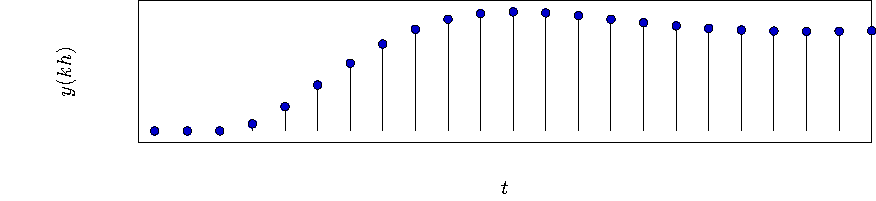
\includegraphics[width=12cm]{second-order-response-example}
\end{center}
\end{enumerate}
\end{block}
\end{frame}
\begin{frame}[label={sec:org97ad0de}]{Tiempo de muestreo}
\begin{block}{Reglas de oro (Åström \& Wittenmark)}
\begin{enumerate}
\setcounter{enumi}{2}
\item Si conocemos la frecuencia de cross-over, podemos eligir el tiempo de muestreo para que el cambio de fase negativo causado por el muestreo y retención no sea entre 5 y 15 grados. El efecto de muestreo y retención es approximadamente un retraso de \(h/2\), \(\mathrm{e}^{-sh/2}\). Resulta la regla
\[ \arg \mathrm{e}^{-i\omega_c h/2} = -\omega_c h/2 \approx \frac{5\pi}{180} \; \text{a} \; \frac{15\pi}{180}\]
\end{enumerate}
\end{block}
\end{frame}

\section{Asignación de polos - Repetición}
\label{sec:org194246d}
\begin{frame}[label={sec:org61ab7d8}]{Diseño por asignación de polos}
\end{frame}
\begin{frame}[label={sec:org29b1f1f}]{Asignación de polos - Un ejemplo}
\begin{center}
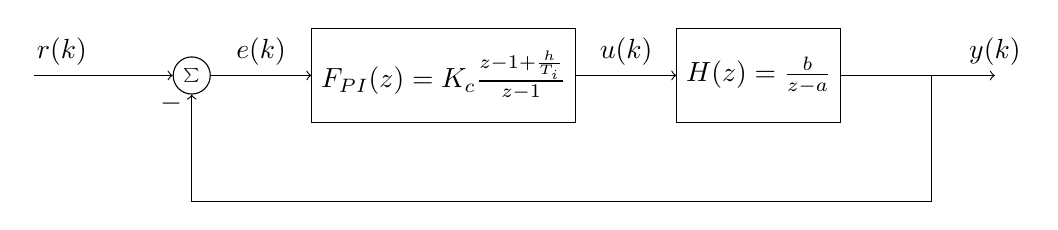
\begin{tikzpicture}
\tikzset{node distance=2cm, 
    block/.style={rectangle, draw, minimum height=12mm, minimum width=14mm},
    sumnode/.style={circle, draw, inner sep=2pt}        
}

  \node[coordinate] (input) {};
  \node[sumnode, right of=input, node distance=20mm] (sum) {\tiny $\sum$};
  \node[block, right of=sum, node distance=32mm] (PI) {$F_{PI}(z) = K_c\frac{z -1 + \frac{h}{T_i}}{z-1}$};
  \node[block,right of=PI, node distance=40mm] (plant) {$H(z) = \frac{b}{z-a}$};
  \node[coordinate, right of=plant, node distance=30mm] (output) {};
  \node[coordinate, right of=plant, node distance=22mm] (measure) {};
  \draw[->] (input) -- node[above, pos=0.2] {$r(k)$} (sum);
  \draw[->] (sum) -- node[above, ] {$e(k)$} (PI);
  \draw[->] (PI) -- node[above] {$u(k)$} (plant);
  \draw[->] (plant) -- node[at end, above] {$y(k)$} (output);
  \draw[->] (measure) -- ++(0,-16mm) -| (sum) node[left, pos=0.96] {$-$};
\end{tikzpicture}
\end{center}

\alert{Queremos un sistema de lazo cerrado criticalmente amortiguado con dos polos en \(z = \alpha, \quad 0 < \alpha < 1\)}
\end{frame}


\begin{frame}[label={sec:orgf194d87}]{Asignación de polos}
\begin{center}
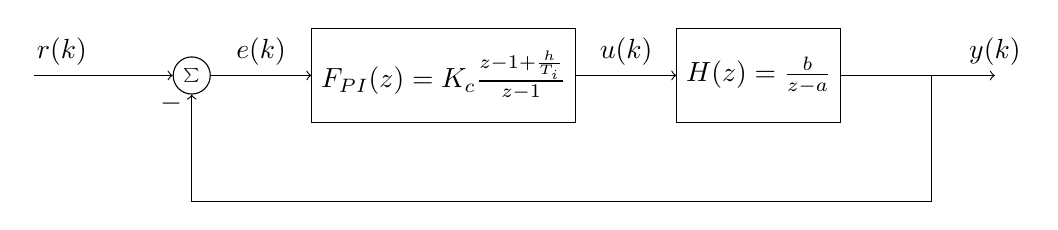
\begin{tikzpicture}
\tikzset{node distance=2cm, 
    block/.style={rectangle, draw, minimum height=12mm, minimum width=14mm},
    sumnode/.style={circle, draw, inner sep=2pt}        
}

  \node[coordinate] (input) {};
  \node[sumnode, right of=input, node distance=20mm] (sum) {\tiny $\sum$};
  \node[block, right of=sum, node distance=32mm] (PI) {$F_{PI}(z) = K_c\frac{z -1 + \frac{h}{T_i}}{z-1}$};
  \node[block,right of=PI, node distance=40mm] (plant) {$H(z) = \frac{b}{z-a}$};
  \node[coordinate, right of=plant, node distance=30mm] (output) {};
  \node[coordinate, right of=plant, node distance=22mm] (measure) {};
  \draw[->] (input) -- node[above, pos=0.2] {$r(k)$} (sum);
  \draw[->] (sum) -- node[above, ] {$e(k)$} (PI);
  \draw[->] (PI) -- node[above] {$u(k)$} (plant);
  \draw[->] (plant) -- node[at end, above] {$y(k)$} (output);
  \draw[->] (measure) -- ++(0,-16mm) -| (sum) node[left, pos=0.96] {$-$};
\end{tikzpicture}
\end{center}

\alert{Ecuación característica}
\begin{align*}
1 + H(z)F_{PI}(z) &= 0\\
(z-1)(z-a) + K_c b (z - 1 + h/T_i) &= 0
\end{align*}
\alert{Polinomio característico}
\[ \underbrace{(z-1)(z-a) + K_c b (z - 1 + h/T_i)}_{\text{parametrizado}} = \underbrace{(z-\alpha)^2}_{\text{deseado}}\]

\alert{¿Cómo podemos determinar los parametros del controlador, \(K_c\) y \(T_i\)?} 
\end{frame}

\begin{frame}[label={sec:org22c7846}]{Asignación de polos - Solución}
\begin{center}
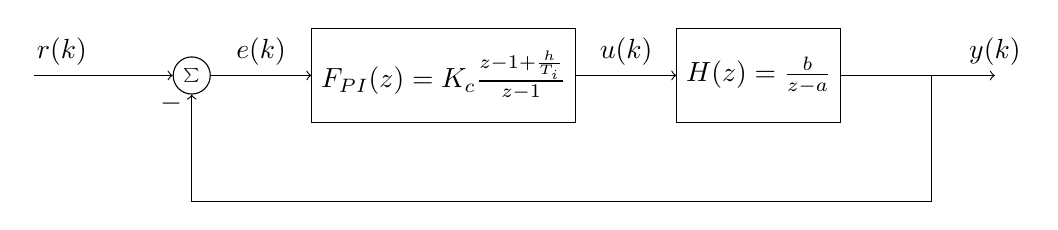
\begin{tikzpicture}
\tikzset{node distance=2cm, 
    block/.style={rectangle, draw, minimum height=12mm, minimum width=14mm},
    sumnode/.style={circle, draw, inner sep=2pt}        
}

  \node[coordinate] (input) {};
  \node[sumnode, right of=input, node distance=20mm] (sum) {\tiny $\sum$};
  \node[block, right of=sum, node distance=32mm] (PI) {$F_{PI}(z) = K_c\frac{z -1 + \frac{h}{T_i}}{z-1}$};
  \node[block,right of=PI, node distance=40mm] (plant) {$H(z) = \frac{b}{z-a}$};
  \node[coordinate, right of=plant, node distance=30mm] (output) {};
  \node[coordinate, right of=plant, node distance=22mm] (measure) {};
  \draw[->] (input) -- node[above, pos=0.2] {$r(k)$} (sum);
  \draw[->] (sum) -- node[above, ] {$e(k)$} (PI);
  \draw[->] (PI) -- node[above] {$u(k)$} (plant);
  \draw[->] (plant) -- node[at end, above] {$y(k)$} (output);
  \draw[->] (measure) -- ++(0,-16mm) -| (sum) node[left, pos=0.96] {$-$};
\end{tikzpicture}
\end{center}
Polinomio característico
\[ \underbrace{z^2 - (1+a -K_cb)z + K_cb(h/T_i - 1) + a}_{\text{parametrizado}} = \underbrace{z^2 -2\alpha z + \alpha^2}_{\text{deseado}}\]

\alert{Los dos polinomios caracteristicos son iguales solamente si cada uno de los coefficientes correspondientes son iguales. Eso nos da dos ecuaciones en los variables desconocidos:}
\begin{align*}
1 + a - K_c b &= 2\alpha \quad \Rightarrow \quad K_c = \frac{1+a-2\alpha}{b}\\
K_cb(h/T_i - 1) + a &= \alpha^2 \quad \Rightarrow \quad \frac{1}{T_i} = \frac{1}{h}\left(1 + \frac{\alpha^2-a}{K_c b}\right) = \frac{1}{h} \left( \frac{(\alpha-1)^2}{1 + a - 2\alpha}\right) 
\end{align*}
\end{frame}


\begin{frame}[label={sec:orga6f4e7b}]{Asignación de polos}
\alert{Ligas}

\href{https://mybinder.org/v2/gh/kjartan-at-tec/mr2007-computerized-control/master?filepath=.\%2Fapproximating-cont-controller\%2Fnotebooks\%2FPole-placement-PI-controller-example.ipynb}{Solución en mybinder}

\href{https://github.com/kjartan-at-tec/mr2007-computerized-control/blob/master/approximating-cont-controller/notebooks/Pole-placement-PI-controller-example.ipynb}{Solución en github}
\end{frame}



\section{Conceptos claves}
\label{sec:orgd785da9}
\begin{frame}[label={sec:orgeca44aa}]{Tres conceptos claves}
\begin{enumerate}
\item Dónde poner los polos del sistem en lazo cerrado
\item La función de \emph{sensibilidad} y la función de \emph{sensibilidad complementaria}
\item Determinar el orden del controlador
\end{enumerate}
\end{frame}

\begin{frame}[label={sec:org1856626}]{Los polos del sistema en lazo cerrado}
Polos complejos en el plano \(s\):
\begin{center}
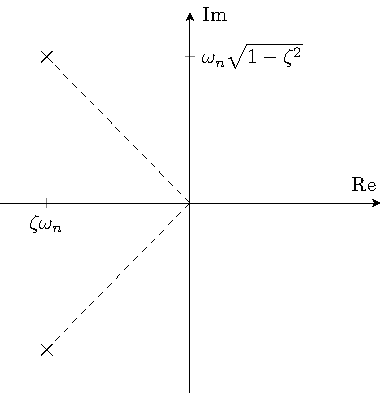
\includegraphics[width=0.45\linewidth]{../../figures/implane-second-order-poles}
\end{center}
\end{frame}

\begin{frame}[label={sec:org3815671}]{Los polos del sistema en lazo cerrado}
Dado especificaciónes de la velocidad y amortiguación del sistema en lazo cerrado
\[ t_s \approx \frac{4}{\zeta\omega_n} < 1 s \qquad \zeta \approx \frac{-\ln (\%OS/100)}{\sqrt{\pi^2 + \ln^2(\%OS/100)}}, \quad OS < 10\%  \]
resulta en 
\[ \zeta > 0.59,  \qquad \zeta\omega_n > 4\]

\begin{center}
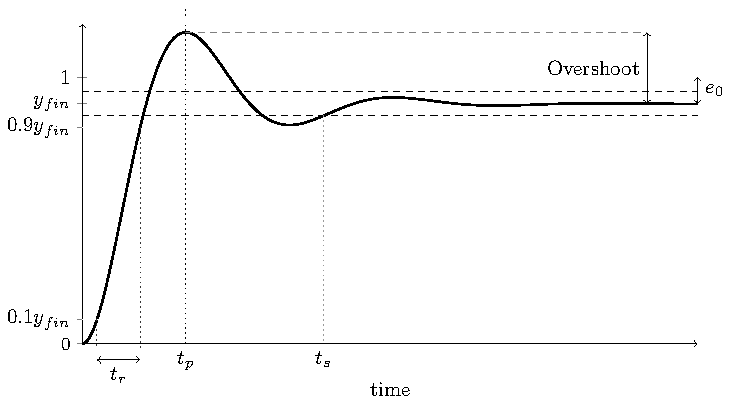
\includegraphics[width=0.6\linewidth]{../../figures/step-response-specifications}
\end{center}
\end{frame}

\begin{frame}[label={sec:org9d67f1d}]{Los polos del sistema en lazo cerrado}
\alert{Actividad} Dado especificaciones \(\zeta > 0.59\) y \(\zeta\omega_n > 4\), marca las regiones en el plano \(s\) y en el plano \(z\) que corresponden a las especificaciones.
\begin{center}
\alert{plano s} \hspace*{0.4\linewidth} \alert{plano z}\\
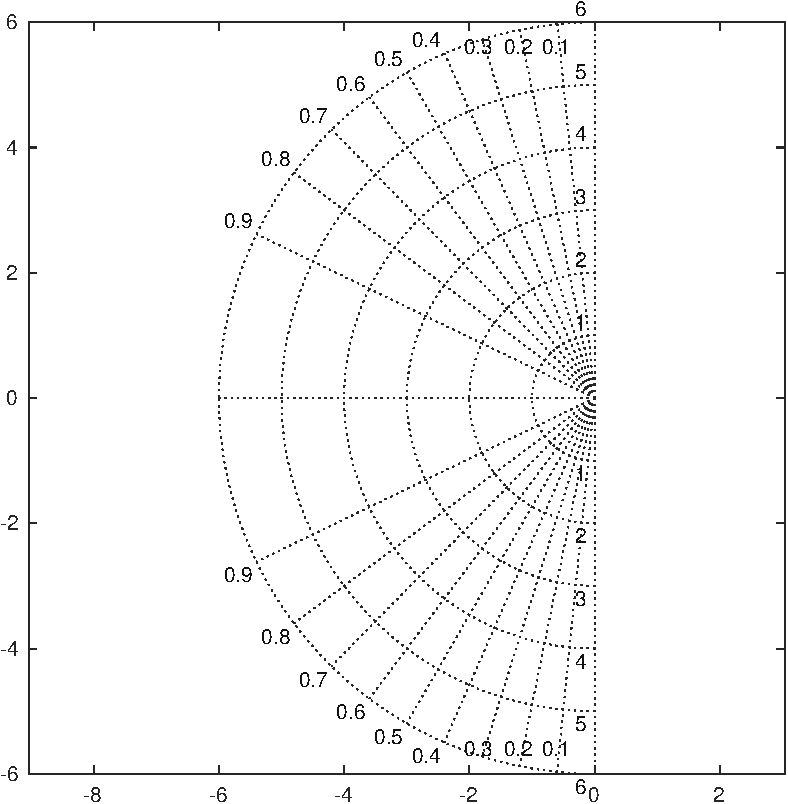
\includegraphics[height=0.61\textheight]{../../figures/sgrid-crop} \hspace*{3mm}
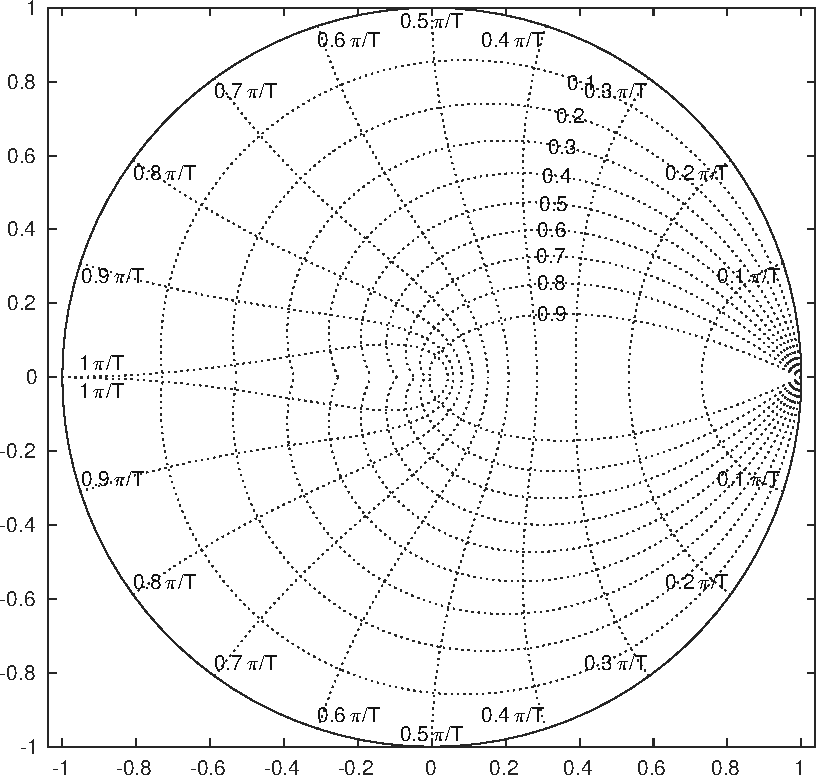
\includegraphics[height=0.6\textheight]{../../figures/zgrid-crop}\\
\end{center}
\end{frame}

\begin{frame}[label={sec:orgbeb7484}]{Las funciones de sensibilidad y sensibilidad complementaria}
\end{frame}
\begin{frame}[label={sec:orgd1adca1}]{Controlador de dos grados de libertad}
\begin{center}
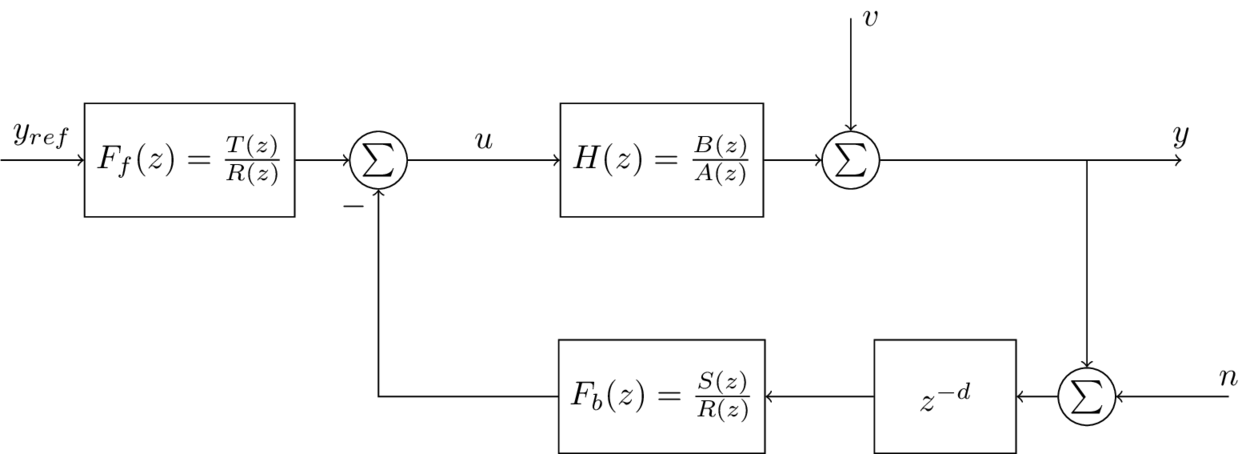
\includegraphics[width=0.8\linewidth]{../../figures/2dof-block-explicit}
\end{center}

\begin{align*}
Y(z) &= G_c(z)U_c(z) + \overbrace{S_s(z)}^{\text{sensib}}V(z) - \overbrace{T_s(z)}^{\text{sens compl}}N(z)\\
     &= \frac{F_f(z)H(z)}{1 + F_b(z)z^{-d}H(z)}U_c(z) + \frac{1}{1 + F_b(z)z^{-d}H(z)}V(z)  - \frac{z^{-d}F_b(z)H(z)}{1 + F_b(z)z^{-d}H(z)}N(z)\\
\end{align*}
\end{frame}

\begin{frame}[label={sec:orgd39eab0}]{Controlador de dos grados de libertad}
\begin{center}
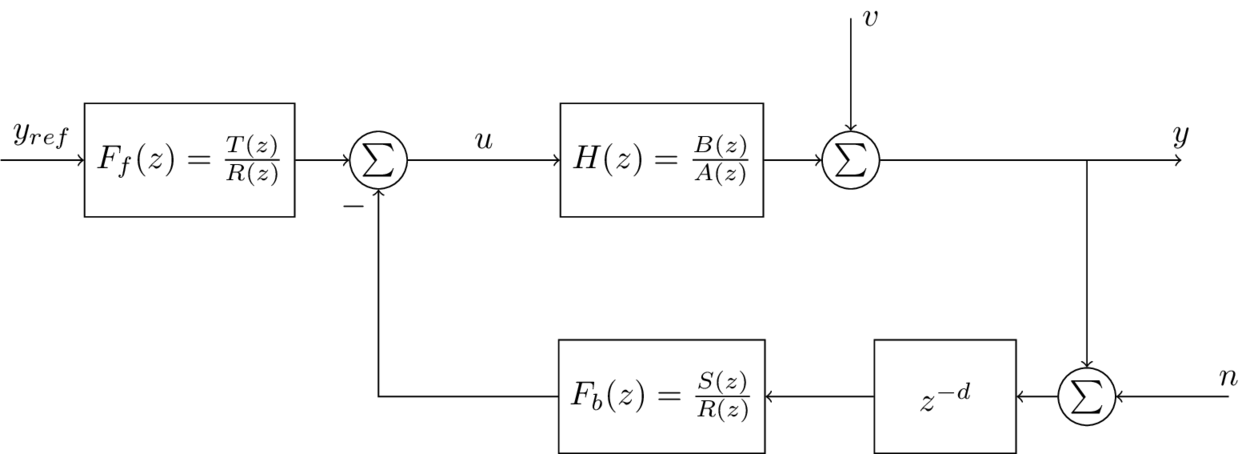
\includegraphics[width=0.7\linewidth]{../../figures/2dof-block-explicit}
\end{center}

\begin{align*}
Y(z)     &= \frac{F_f(z)H(z)}{1 + z^{-d}F_b(z)H(z)}U_c(z) + \overbrace{\frac{1}{1 + z^{-d}F_b(z)H(z)}}^{S_s(z)}V(z)  - \overbrace{\frac{z^{-d}F_b(z)H(z)}{1 + z^{-d}F_b(z)H(z)}}^{T_s(z)}N(z)\\
\end{align*}

\alert{Evidentemente} \(S_s(z) + T_s(z) = 1\) \alert{Conclusion:} Hay que encontrar un equilibrio entre rechazo a perturbaciones y rechazo a ruido de medida.
\end{frame}

\begin{frame}[label={sec:org5c57d5f}]{Sensibilidad y sensibilidad complementaria}
\alert{Actividad} Marca en el plano complejo los puntos indicados en el diagrama de Bode para ambos sistemas \(S_s(z)\) y \(T_s(z)\). Verifica que la suma vectorial de los puntos es 1.
\begin{center}
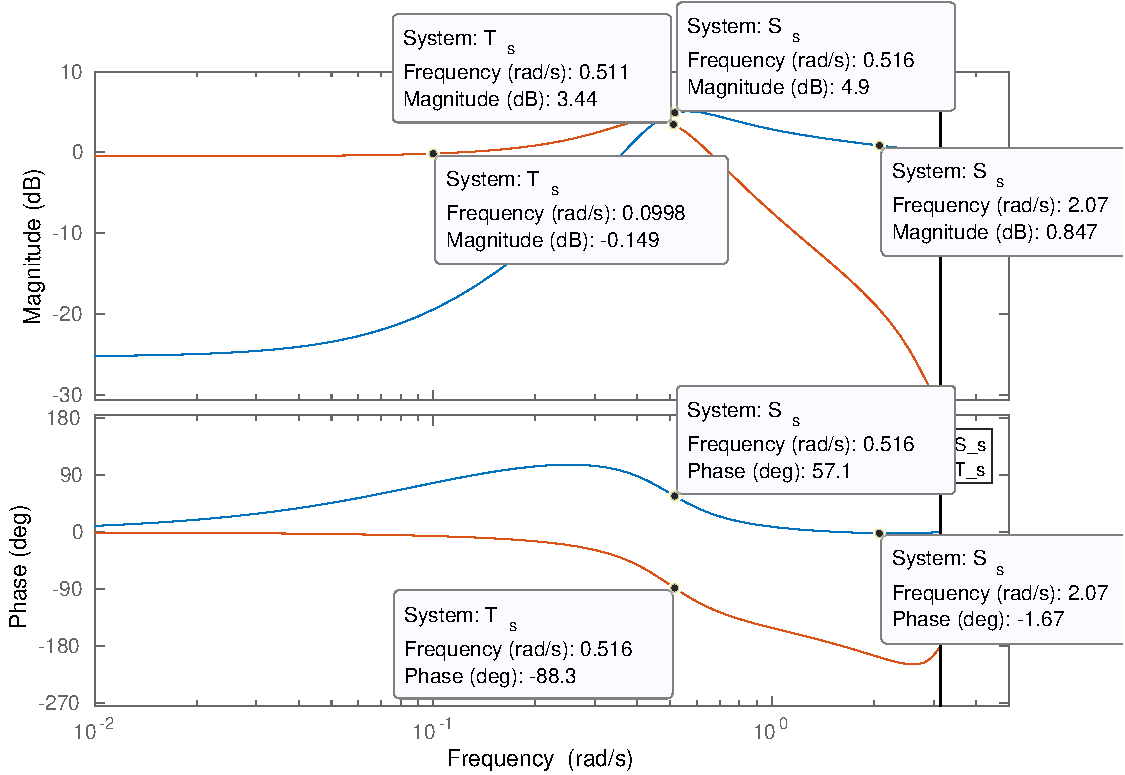
\includegraphics[width=0.7\linewidth]{../matlab/bode-sensitivity-exercise-crop}
\end{center}
\end{frame}

\begin{frame}[label={sec:org2b09be9}]{Sensibilidad y sensibilidad complementaria}
\pgfmathsetmacro{\Smag}{0.12}
\pgfmathsetmacro{\Sarg}{70}
\pgfmathsetmacro{\Sreal}{\Smag*cos(\Sarg)}
\pgfmathsetmacro{\Sim}{\Smag*sin(\Sarg)}
\pgfmathsetmacro{\Tmag}{0.98}
\pgfmathsetmacro{\Targ}{-6}
\pgfmathsetmacro{\Treal}{\Tmag*cos(\Targ)}
\pgfmathsetmacro{\Tim}{\Tmag*sin(\Targ)}
\alert{Punto 1:} \(\omega=0.1\), \(T_s(0.1) = 10^{-0.149/20}\mathrm{e}^{-i6^o} = 0.98\mathrm{e}^{-i6^o} = 0.97 - i0.1\), \(S_s(0.1) = 10^{-18/20}\mathrm{e}^{i70^o} = 0.12\mathrm{e}^{i70^o} = 0.04 + i0.11\)
\begin{center}
  \begin{tikzpicture}[scale=1.6]

    \draw[->] (-2, 0) -- (2, 0) node[below] {Re};
    \draw[->] (0,-2) -- (0,2) node[left] {Im};
    \node[circle, fill, orange, inner sep= 1pt] (Tone) at (\Treal, \Tim) {};
    \draw[thin, ->, orange] (0,0) to (Tone);
    \node[circle, fill, blue!80, inner sep= 1pt] (Sone) at (\Sreal, \Sim) {};
    \draw[thin, ->, blue!80] (0,0) to (Sone);
    \draw (1,0) -- (1,-0.05) node[below] {1};
    \draw (-1,0) -- (-1,-0.05) node[below] {-1};
    \draw (0,1) -- (-0.05,1) node[left] {i};
    \draw (0,-1) -- (-0.05,-1) node[left] {-i};
  \end{tikzpicture}
\end{center}
\end{frame}

\begin{frame}[label={sec:orgcb6a47a}]{Sensibilidad y sensibilidad complementaria -  Solución}
\end{frame}
\begin{frame}[label={sec:orgf5f0646}]{Sensibilidad y sensibilidad complementaria -  Solución}
\pgfmathsetmacro{\Smag}{0.12}
\pgfmathsetmacro{\Sarg}{70}
\pgfmathsetmacro{\Tmag}{0.98}
\pgfmathsetmacro{\Targ}{-6}
\pgfmathsetmacro{\Treal}{\Tmag*cos(\Targ)}
\pgfmathsetmacro{\Tim}{\Tmag*sin(\Targ)}

\pgfmathsetmacro{\Smagtwo}{0.12}
\pgfmathsetmacro{\Sargtwo}{70}
\pgfmathsetmacro{\Srealtwo}{\Smagtwo*cos(\Sargtwo)}
\pgfmathsetmacro{\Simtwo}{\Smag*sin(\Sarg)}
\pgfmathsetmacro{\Tmagtwo}{0.98}
\pgfmathsetmacro{\Targtwo}{-6}

\begin{center}
  \begin{tikzpicture}[scale=1.6]

    \draw[->] (-2, 0) -- (2, 0) node[below] {Re};
    \draw[->] (0,-2) -- (0,2) node[left] {Im};
    \draw (1,0) -- (1,-0.05) node[below] {1};
    \draw (-1,0) -- (-1,-0.05) node[below] {-1};
    \draw (0,1) -- (-0.05,1) node[left] {i};
    \draw (0,-1) -- (-0.05,-1) node[left] {-i};
 

    \foreach \Tmag/\Targ/\nn in {-0.149/-6/1, 3.44/-88/2, -19/-196/3} {
       \pgfmathsetmacro{\Treal}{pow(10,\Tmag/20)*cos(\Targ)}
       \pgfmathsetmacro{\Tim}{pow(10,\Tmag/20)*sin(\Targ)}
       \node[circle, fill, orange, inner sep= 1pt] (Tone) at (\Treal, \Tim) {};
           \draw[thin, ->, orange] (0,0) to (Tone) node[right] {\tiny \nn};
	   }
    \foreach \Smag/\Sarg/\nn in {-18/78/1, 4.9/57/2, 0.85/-1.67/3} {
       \pgfmathsetmacro{\Sreal}{pow(10,\Smag/20)*cos(\Sarg)}
       \pgfmathsetmacro{\Sim}{pow(10,\Smag/20)*sin(\Sarg)}
       \node[circle, fill, blue!80, inner sep= 1pt] (Sone) at (\Sreal, \Sim) {};
           \draw[thin, ->, blue!80] (0,0) to (Sone) node[right] {\tiny \nn};
	   }

    %\node[circle, fill, blue!80, inner sep= 1pt] (Sone) at (\Sreal, \Sim) {};
    %\draw[thin, ->, blue!80] (0,0) to (Sone);
  \end{tikzpicture}
\end{center}
\end{frame}

\section{Cancelación de polos del observador}
\label{sec:org2fe25ec}
\begin{frame}[label={sec:orgb7ed41e}]{Controlador de dos grados de libertad}
\begin{center}
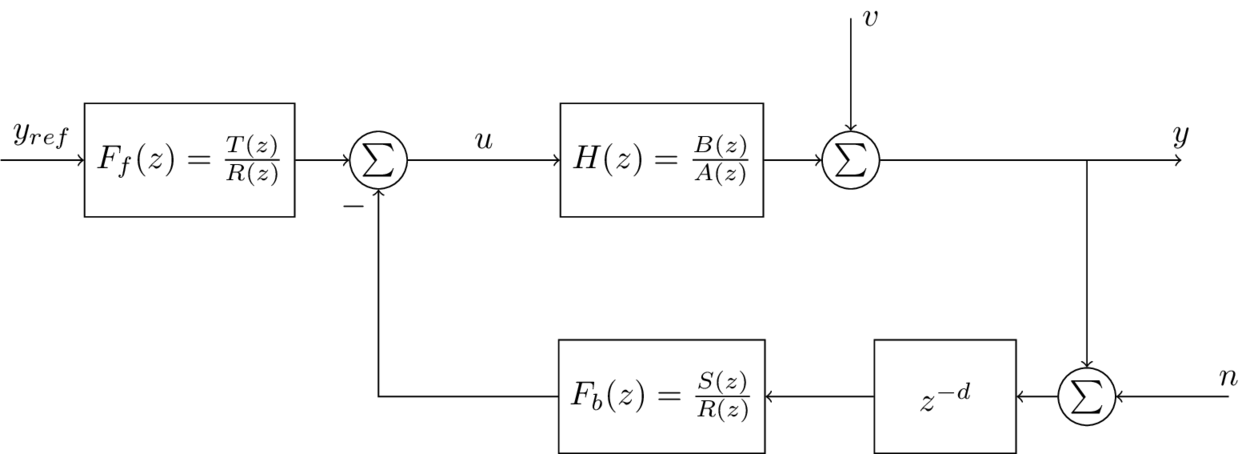
\includegraphics[width=0.7\linewidth]{../../figures/2dof-block-explicit}
\end{center}

\begin{align*}
Y(z) &= \frac{T(z)B(z)z^d}{z^dA(z)R(z) + B(z)S(z)}U_c(z) + \frac{A(z)R(z)z^d}{z^dA(z)R(z) + B(z)S(z)}V(z)\\ & \qquad\qquad\qquad - \frac{S(z)B(z)}{z^dA(z)R(z) + B(z)S(z)}N(z)
\end{align*}
\end{frame}




\begin{frame}[label={sec:orgaf2fb5e}]{Controlador de dos grados de libertad}
\begin{align*}
Y(z) &= \frac{T(z)B(z)z^d}{z^dA(z)R(z) + B(z)S(z)}U_c(z) + \frac{A(z)R(z)z^d}{z^dA(z)R(z) + B(z)S(z)}V(z)\\ & \qquad\qquad\qquad - \frac{S(z)B(z)}{z^dA(z)R(z) + B(z)S(z)}N(z)\\
     &= \frac{T(z)B(z)z^d}{A_c(z)A_o(z)}U_c(z) + \frac{A(z)R(z)z^d}{A_c(z)A_o(z)}V(z)- \frac{S(z)B(z)}{A_c(z)A_o(z)}N(z), \quad \text{elige}\, T(z) = t_0A_o(z)\\
     &= \frac{t_0B(z)z^d}{A_c(z)}U_c(z) + \frac{A(z)R(z)z^d}{A_c(z)A_o(z)}V(z)- \frac{S(z)B(z)}{A_c(z)A_o(z)}N(z)
\end{align*}
\end{frame}

\begin{frame}[label={sec:org72ddd7f}]{Controlador de dos grados de libertad}
\begin{center}
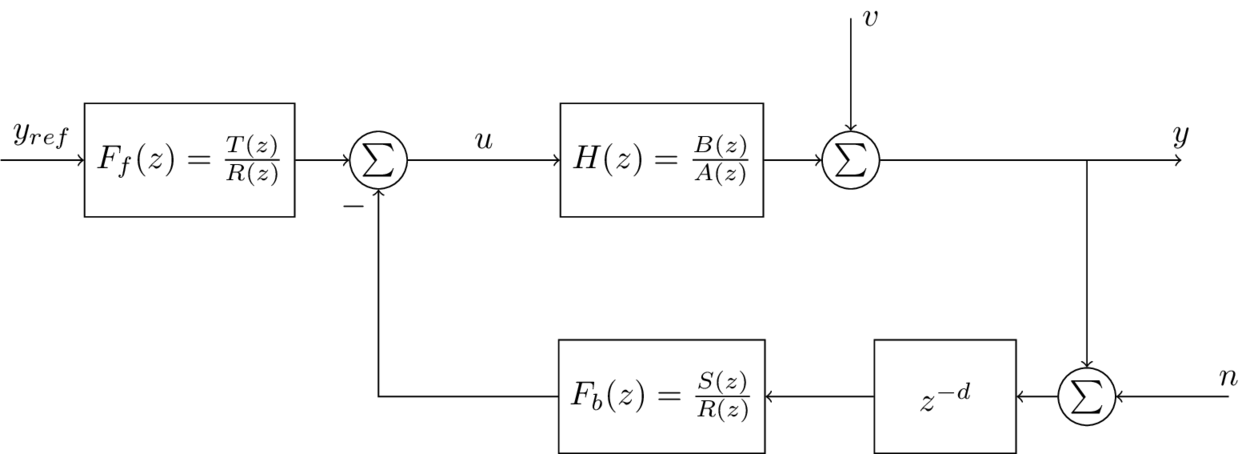
\includegraphics[width=0.7\linewidth]{../../figures/2dof-block-explicit}
\end{center}
\begin{align*}
Y(z) &= \frac{t_0B(z)z^d}{A_c(z)}U_c(z) + \frac{A(z)R(z)z^d}{A_c(z)A_o(z)}V(z)- \frac{S(z)B(z)}{A_c(z)A_o(z)}N(z)
\end{align*}
\end{frame}

\begin{frame}[label={sec:org29d1711}]{Controlador de dos grados de libertad}
\begin{center}
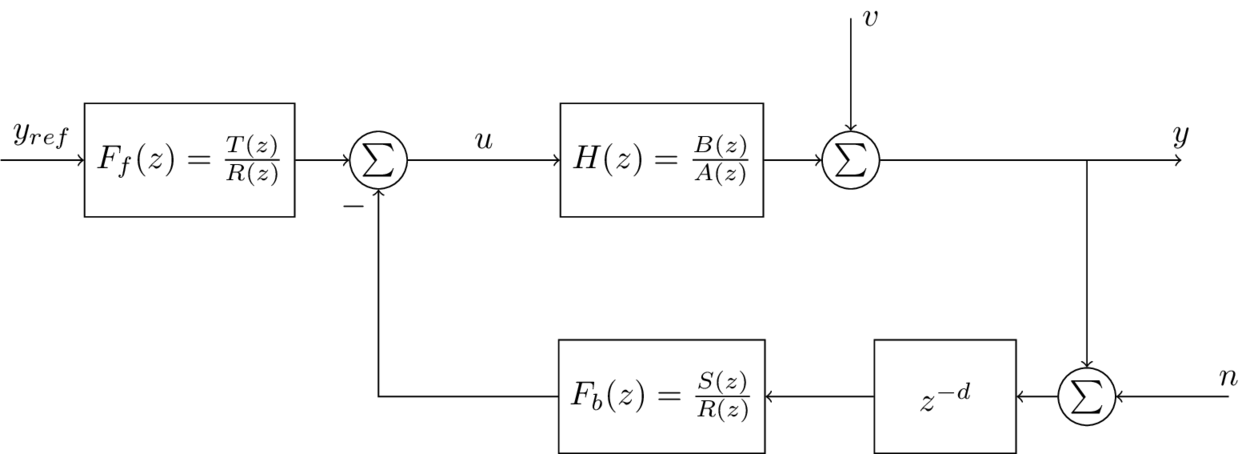
\includegraphics[width=0.7\linewidth]{../../figures/2dof-block-explicit}
\end{center}
\begin{align*}
Y(z) &= \frac{t_0B(z)z^d}{A_c(z)}U_c(z) + \frac{A(z)R(z)z^d}{A_c(z)A_o(z)}V(z)- \frac{S(z)B(z)}{A_c(z)A_o(z)}N(z)
\end{align*}
\alert{Conclusiones} 1) Hay una separación parcial entre seguimiento de la referencia y rechazo a perturbaciones. 2) Se puede usar los polos correspondientes a las raíces de \(A_o(z)\) para afinar el rechazo a perturbaciones contra rechazo a ruido de medida. 
\end{frame}


\section{RST}
\label{sec:org427d3b8}

\begin{frame}[label={sec:orgcbf1ef7}]{Procedimiento - asignación de polos}
Dado modelo del proceso \(H(z)=\frac{B(z)}{A(z)}\), y specificaciones de polos deseados del sistema en lazo cerrado \(A_{cl}(z) = (z-\alpha_1)(z-\alpha_2) \cdots (z-\alpha_{n_c})\)
\begin{enumerate}
\item Determina la ecuación diofántica
\[ A(z)R(z)z^{d} + B(z)S(z) = A_{cl}(z) \]
y el orden adecuado del controlador, con \(\deg S = \deg R\).
\item Factoriza el polinomio caracteristico del lazo cerrado \(A_{cl}(z) = A_c(z)A_o(z)\), donde \(n_{A_o} = n_R\).
\item Determina polinomios \(R(z)\) y \(S(z)\) que satisfican
\[ A(z)R(z)z^{d} + B(z)S(z) = A_{cl}(z) \]
\end{enumerate}
\end{frame}

\begin{frame}[label={sec:orgee46d18}]{Procedimiento}
Dado modelo del proceso \(H(z)=\frac{B(z)}{A(z)}\), y specificaciones de polos deseados del sistema en lazo cerrado \(A_{cl}(z) = (z-\alpha_1)(z-\alpha_2) \cdots (z-\alpha_{n_c})\)
\begin{enumerate}
\setcounter{enumi}{3}
\item Elige
\[T(z) = t_0 A_o(z),\] donde \(t_0 = \frac{A_c(1)}{B(1)}\).
\end{enumerate}

Resulta la ley de control 
\[ R(q) u(k) = T(q)u_c(k) - S(q)y(k). \]
y la respuesta en lazo cerrado a la señal de referencia
\[ A_c(q)y(k) = t_0 B(q) u_c(k). \]
\end{frame}

\begin{frame}[label={sec:org6c36087}]{Determinando el orden del controlador}
Tenemos la ecuación diafóntica
   \[ A(z)R(z)z^{d} + B(z)S(z) = A_{cl}(z) \qquad (*) \]
y el controlador
\[F_b(z) = \frac{S(z)}{R(z)} = \frac{s_0z^n + s_1z^{n-1} + \cdots + s_n}{z^n + r_1 z^{n-1} + \cdots + r_n}\]
\alert{¿Cómo decidir el orden del controlador?} Nota
\begin{itemize}
\item el controlador tiene \(n+n+1 = 2\deg R + 1\) parámetros desconocidos
\item el lado izquierdo de \((*)\) tiene el grado \(\deg \big(A(z)R(z)z^d + B(z)S(z)\big) = \deg A + \deg R + d\)
\item la ecuación diofántica da un numero de ecuaciones (no-triviales) igual a su grado, al poner coeficientes de los dos lados iguales.

\alert{\(\Rightarrow\;\)Elige \(\deg R\) que satisface \(2\deg R + 1 = \deg A + \deg R + d\)}
\end{itemize}
\end{frame}


\section{Ejemplo}
\label{sec:org7994b02}
\begin{frame}[label={sec:org2b1ef95}]{Ejemplo - Control de nivel de una presa}
\begin{center}
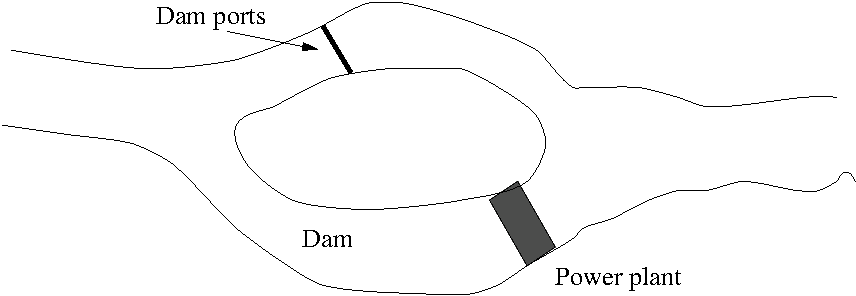
\includegraphics[width=0.5\linewidth]{../../figures/kraftverk}
\end{center}

\alert{Objetivo} Obtener un sistema en lazo cerrado con polos en \(z=0.9\).
\end{frame}

\begin{frame}[label={sec:org244005e}]{Ejemplo - Control de nivel de una presa}
\begin{center}
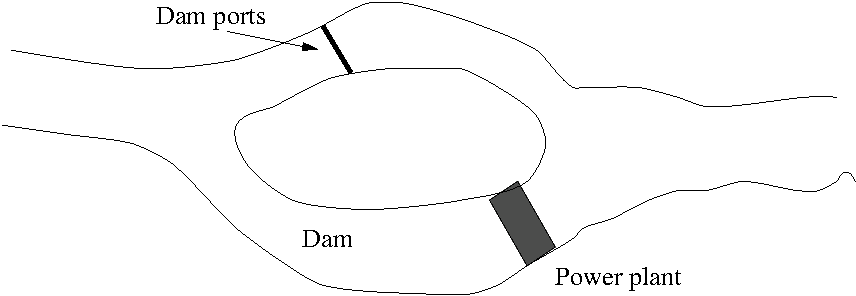
\includegraphics[width=0.5\linewidth]{../../figures/kraftverk}
\end{center}

\alert{Dinámica del proceso}

\begin{center}
  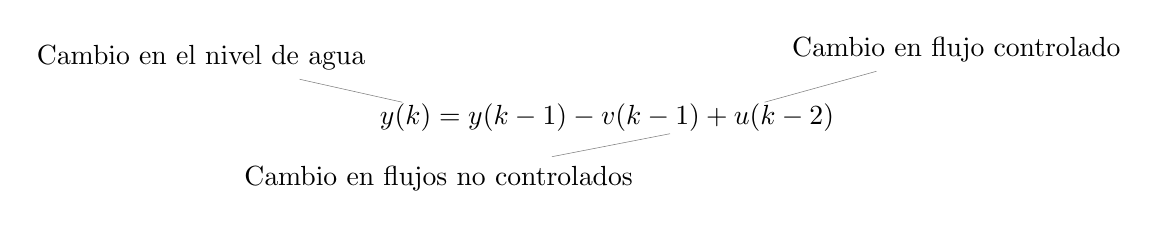
\begin{tikzpicture}
    \node at (0,0) {$y(k) = y(k-1) -v(k-1) + u(k-2)$};
    \node[coordinate, pin=140:{Cambio en el nivel de agua}] at (-2.6,0.2) {};
    \node[coordinate, pin=-140:{Cambio en flujos no controlados}] at (0.8,-0.2) {};
    \node[coordinate, pin=60:{Cambio en flujo controlado}] at (2,0.2) {};
\end{tikzpicture}
\end{center}

\alert{Actividad} ¿Cuál es la funcion de transferencia correcta?

\begin{center}
\begin{tabular}{lll}
1: \(H(z) = \frac{z}{z-1}\) & 2: \(H(z)=\frac{1}{z-1}\) & 3: \(H(z)=\frac{1}{z(z-1)}\)\\
\end{tabular}
\end{center}
\end{frame}

\begin{frame}[label={sec:orgb2f1ba3}]{Ejemplo - Control de nivel de una presa}
Dado proceso \(H(z) = \frac{B(z)}{A(z)} = \frac{1}{z(z-1)}\) y polos deseados en \(z=0.9\).

\begin{enumerate}
\item Ecuación diofántica \(A(z)R(z)z^d + B(z)S(z) = A_{cl}(z)\)
\[ z(z-1)R(z) + S(z) = A_{cl}(z)\]
El orden del controlador es 
\[\deg R = \deg A + d - 1 = 2-1 = 1, \quad \Rightarrow \quad F_b(z)=\frac{S(z)}{R(z)} = \frac{s_0z + s_1}{z + r_1}\]
\item Tenemos la ecuación diofántica
\[ z(z-1)(z+r_1) + s_0z + s_1 = A_{cl}(z)\]
El grado de \(A_{cl}(z)\) es 3. Eligimos \(A_o(z) = z\),  ( \(\deg A_o = \deg R\)) 
\[ A_{cl}(z) = A_o(z) A_c(z) = z(z-0.9)^2\]
\end{enumerate}
\end{frame}

\begin{frame}[label={sec:orgec59c59}]{Ejemplo - Control de nivel de una presa}
\begin{enumerate}
\setcounter{enumi}{2}
\item De la ecuación diofántica \[ z(z-1)(z+r_1) + s_0z + s_1 = z(z-0.9)^2\]
\[ z^3 + (r_1-1)z^2 - r_1z + s_0z + s_1 = z^3 -1.8z^2 + 0.81z\]
Obtenemos las ecuaciones 
\begin{align*}
\begin{cases} z^2 &: \quad r_1-1 = -1.8\\
z^1 &: \quad -r_1 + s_0 = 0.81\\
z^0 &: \quad s_1 = 0
\end{cases}
\quad \Rightarrow \quad 
\begin{cases} r_1 &= -0.8\\ s_0 &= 0.01\\ s_1 &=0 \end{cases}
\end{align*}
\[F_b(z) = \frac{0.01z}{z - 0.8}\]
\end{enumerate}
\end{frame}

\begin{frame}[label={sec:org072c55a}]{Ejemplo - Control de nivel de una presa}
\begin{enumerate}
\setcounter{enumi}{3}
\item Tenemos \(A_o(z) = z\), entonces 
\[T(z) = t_0A_o(z) = t_0z\]
\[G_c(z) = \frac{T(z)B(z)}{A_o(z)A_c(z)} = \frac{t_0 B(z)}{A_c(z)}, \quad \text{queremos}\, G_c(1)=1\]
\[ t_0 = \frac{A_c(1)}{B(1)} = \frac{(1-0.9)^2}{1} = 0.01\]
\end{enumerate}

\alert{Ley de conctrol}
\[R(\shift) u(kh) = T(\shift)u_c(kh) - S(\shift)y(kh)\]
\[ (\shift - 0.8)u(kh) = 0.01\shift u_c(kh) - 0.01\shift y(kh)\]
\[ u(kh+h) = 0.8u(kh) + 0.01 u_c(kh+h) - 0.01y(kh+h)\]
\end{frame}
\end{document}